% Chapter Template

\chapter{Marco Teórico} % Main chapter title

\label{Chapter2} % Change X to a consecutive number; for referencing this chapter elsewhere, use \ref{ChapterX}

\lhead{Capítulo 2. \emph{Marco Teórico}} % Change X to a consecutive number; this is for the header on each page - perhaps a shortened title

\section{Internet of Things(IoT)}

\section{Sistema Embebido}
\subsection{Elección del Hardware}
\subsection{Firmware}

\section{Protocolos de Comunicación}
\subsection{mDNS y DNS-SD}
\subsection{WiFi}
\subsection{HTTP}
\section{API}
\subsection{RPC - Remote Procedure Call}
\subsection{JSON}
\subsection{JSON-RPC}
Hypertext Transfer Protocol es un protocolo de capa de aplicación 7mo nivel según el modelo OSI o el cuarto nivel del stack TCP/IP. Este protocolo permite las transferencias de información en la World Wide Web. HTTP define la sintaxis y la semántica que utilizan los elementos de software de la arquitectura web (clientes, servidores, proxies) para comunicarse. HTTP es un protocolo sin estado, es decir, no guarda ninguna información sobre conexiones anteriores.
Es un protocolo orientado a transacciones y sigue el esquema petición-respuesta entre un cliente y un servidor. El cliente realiza una petición enviando un mensaje, con cierto formato al servidor. 
\subsection{Mensajes}
Los mensajes HTTP se envían en en texto plano y tienen la siguiente estructura:

\begin{itemize}
	\item Línea inicial.
	\subitem solicitud: acción requerida por el cliente con el método de petición y la url del recurso y la versión HTTP del cliente.
	\subitem respuesta: versión de HTTP del servidor seguido del código de respuesta.
	\item Cabeceras:Lista de metadatos estandarizados que finaliza con una linea en blanco.
	\item Cuerpo del mensaje.
\end{itemize}

\subsubsection{Digest Authentication}

\subsection{MQTT}
\subsection{TLS-SSL}

\section{Aplicación Cliente}
Para realizar la primera implementación de la aplicación cliente se eligió la plataforma de desarrollo para dispositivos android, más precisamente teléfonos inteligentes y tabletas.

El objetivo principal de emplear una estructura fija para la implementación del proyecto es utilizar un único "lenguaje arquitectónico" que resulte familiar a los integrantes de un posible equipo de desarrollo así como transversal tanto para la implementación android, iOS o cualquier otra plataforma que pueda aparecer durante la vida útil del producto. De esta manera no es necesario pagar un costo demasiado alto al incluir una implementación del mismo sistema para una plataforma distinta. 
Los equipos de cada una de estas implementaciones podrán discutir aspectos de diseño, validar reglas de negocio y evacuar dudas sin tener en cuenta los detalles de las plataformas, así mismo será más fácil conservar coherencia y mostrar armonía entre las implementaciones nativas para dichas plataformas.

\section{Uncle Bob Clean Architecture}

También conocida como arquitectura de capas (onion architecture). El punto principal de este enfoque es que la lógica de negocio, también conocido como dominio, está en el centro del universo (Al medio entre las entradas del sistema y las salidas)\cite{clean_bob}.
%\todo expandi esto negro
\subsection{Dominio Transparente}
Cuando se listen los directorios de un proyecto que cumple con los lineamiento de esta arquitectura, con tan solo leer el nombre de las carpetas debería ser posible casi de inmediato tener una idea de qué se trata esta aplicación, independientemente de la tecnología. Todo lo demás es un \emph{detalle de implementación}\cite{clean_five}. \\
Por ejemplo, la persistencia es un detalle. Definir una interfaz con el objetivo de establecer la responsabilidad con un contrato (Contrato de Persistencia),  de esta forma uno podría implementar de una manera rápida e insuficiente una estrategia de persistencia en memoria RAM y no pensar en ello demasiado sino hasta que la lógica de negocio esté completamente definida. Una vez definidos los requerimientos de persistencia y verificados con el cliente, se puede proceder a tomar una decisión definitiva de \textbf{cómo} deberán persistirse los datos.\\ 
Almacenamiento en una base de datos local, comunicación remota con un servicio REST, almacenamiento sobre el sistema de archivos, ante este panorama incluso sería razonable pensar el planteo de la creación de un esquema de cache, y sin embargo no es poco frecuente que luego de la elicitación de requerimientos resulte que el sistema no tiene que persistir ningún resultado en absoluto.\\ 
En una frase: \textit{las capas internas contienen lógica de negocios, las capas externas contienen detalles de implementación}.
Adicionalmente esta arquitectura debe cumplir con un conjunto de características:

\begin{itemize}
	\item Regla de dependencia
	\item Abstracción
	\item Comunicación entre capas
\end{itemize}

\subsection{Regla de Dependencias}
La regla de dependencia se ilustra en la figura ~\ref{fig:Diagrama_clasico}:

\begin{figure}[htbp]
	\centering
	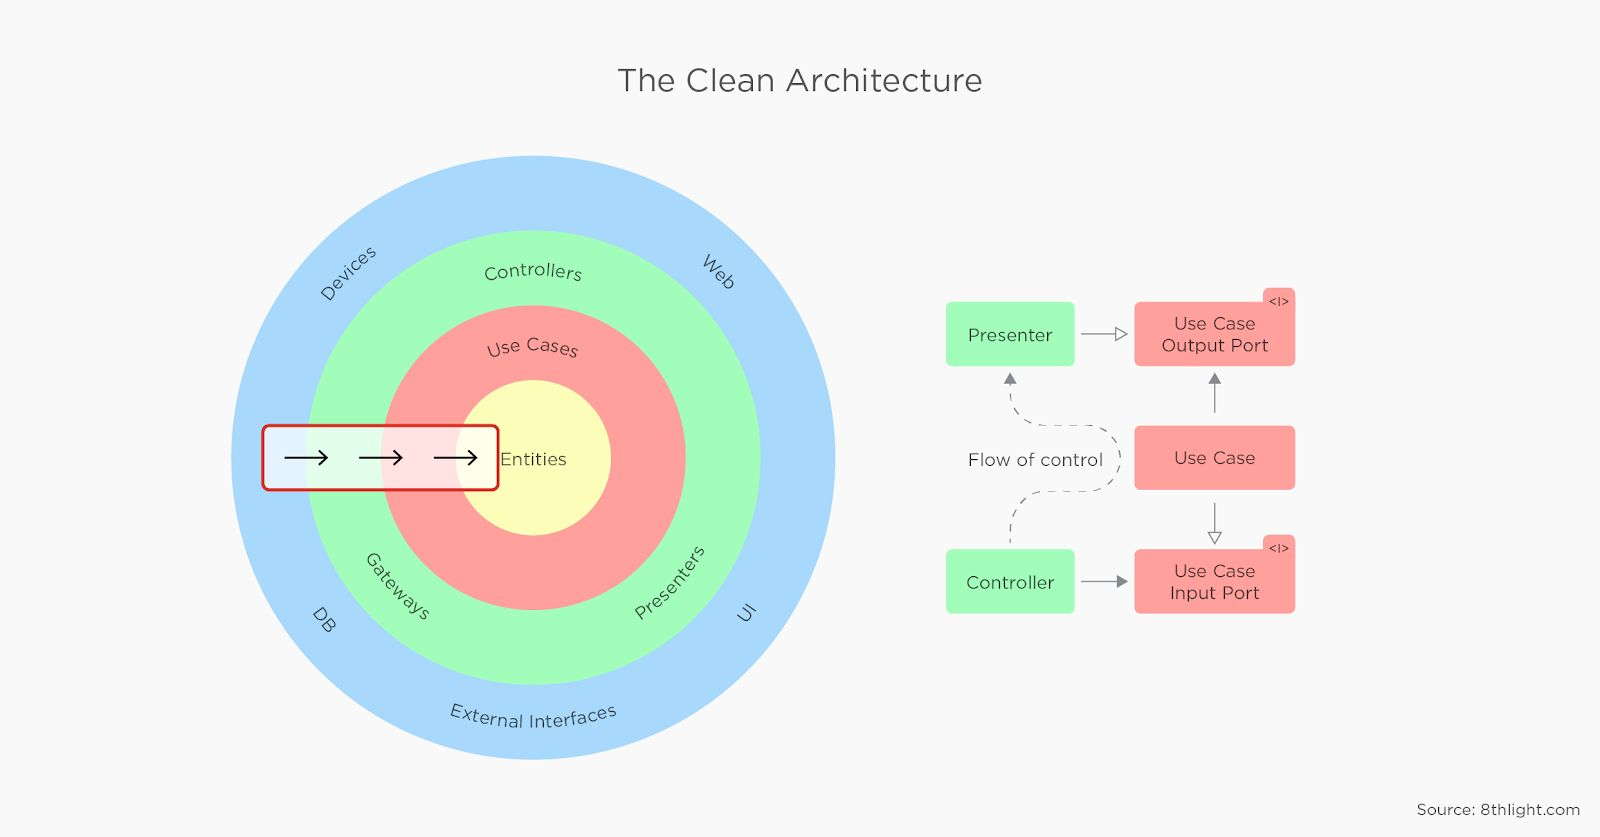
\includegraphics[width=1\textwidth]{Figures/-001.png}
	\rule{35em}{1pt}
	\caption[Principio de Dependecias]{Esquema de dependencias para una arquitectura en capas.}
	\label{fig:Diagrama_clasico}
\end{figure}


Las capas externas deben depender de las capas internas. Permaneciendo en el centro las entidades del dominio inmediatamente seguidas por los objetos que encapsulan la lógica de negocio y que tienen acceso a tal dominio.  Se muestran tres flechas en un recuadro rojo que representan el sentido de las dependencias. En lugar de "depende", tal vez sea mejor usar términos como ''ve'', ''conoce'' o ''está consciente de...''. En estos términos, las capas externas ven, conocen y son conscientes de las capas internas, pero las capas internas no ven ni conocen, ni son conscientes de, las capas externas. Como dijimos anteriormente, las capas internas contienen lógica de negocios y las capas externas contienen detalles de implementación. Combinado con la regla de dependencia, se deduce que la lógica de negocio no ve, ni conoce, detalles de implementación.

No existe una única forma de implementar esta regla, dependerá del encargado del proyecto. Una estrategia consiste en colocar las clases de cada capa en paquetes diferentes, poniendo especial cuidado en no importar paquetes ''externos'' en paquetes ''internos''. Sin embargo, si algún programador del equipo no es consciente del principio de dependencias, nada les impediría romperlo. Un mejor enfoque sería separar las capas en diferentes módulos de construcción independiente, y ajustar las dependencias en el archivo de construcción para que la capa interna simplemente no pueda utilizar la capa externa, sin embargo este enfoque implica un exhaustivo conocimiento de la herramienta de construcción de la plataforma para la que se está desarrollando.

\subsection{Principio de Abstracción}
El principio de la abstracción ya se ha insinuado antes. Postula que a medida que se están moviendo hacia el centro del diagrama, las implementaciones se vuelven más abstractas, agnósticas de plataformas y frameworks. Eso tiene sentido, como lo repetimos anteriormente el círculo interno contiene lógica de negocios y el círculo exterior contiene detalles de implementación.

\begin{figure}[htbp]
	\centering
	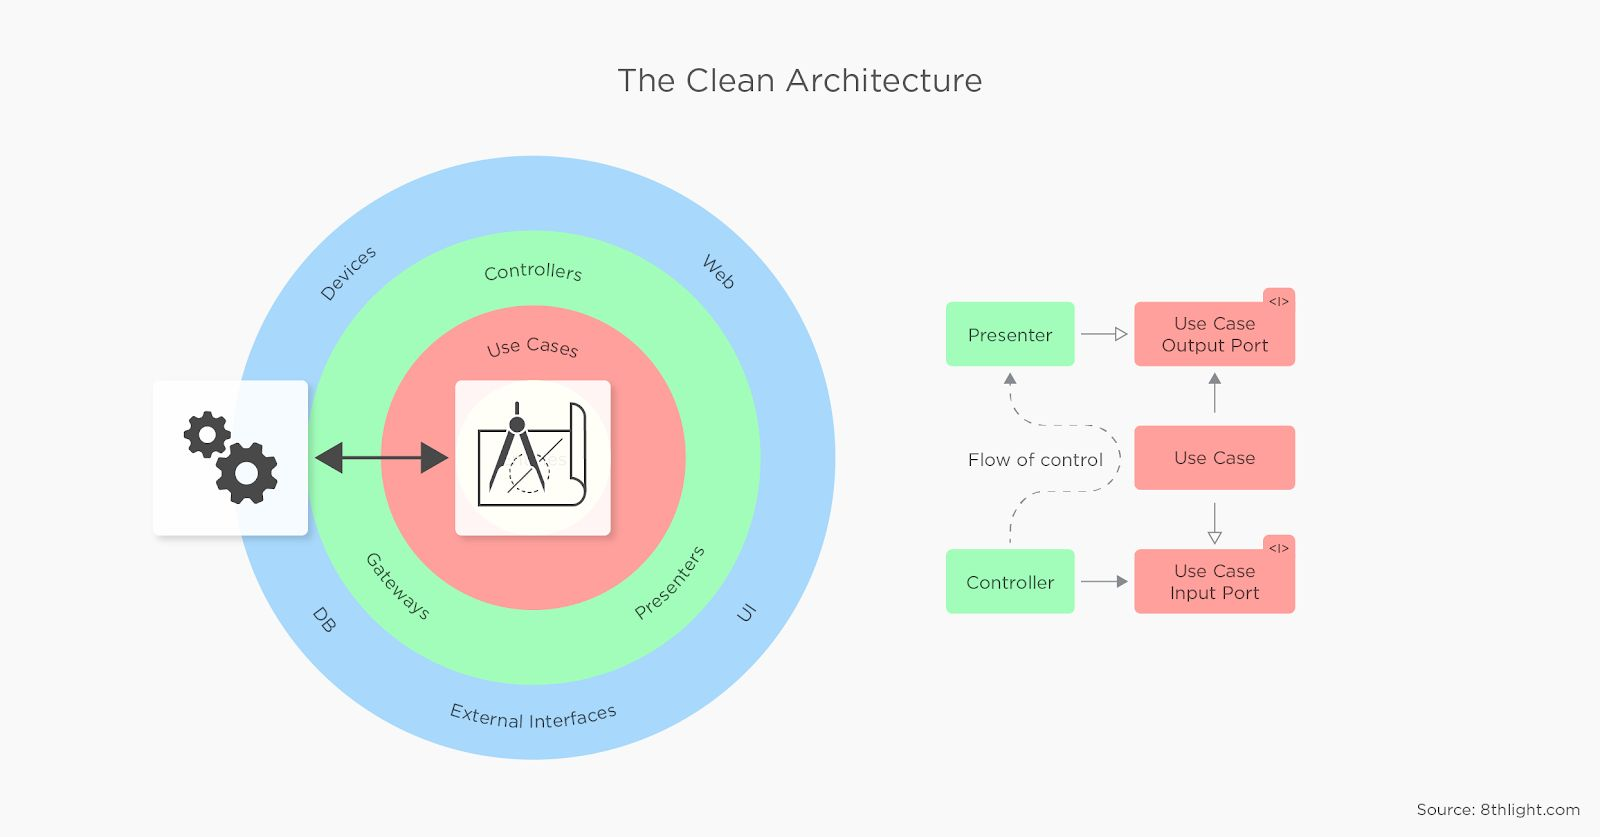
\includegraphics[width=1\textwidth]{Figures/-002.png}
	\rule{35em}{1pt}
	\caption[Abstraction Principle]{Principio de Abstracción en una arquitectura por capas.}
	\label{fig:C2_PA}
\end{figure}

Incluso puede plantearse el mismo componente lógico dividido entre varias capas, como se muestra en el diagrama ~\ref{fig:C2_PA}. La parte más abstracta se puede definir en la capa interna, y la parte más concreta en la capa externa.

De esta manera, la lógica de negocios podría producir como un efecto secundario que se muestren notificaciones del sistema por ejemplo, pero no sabe nada acerca de los detalles de la implementación (cómo se implementan las notificaciones para una plataforma dada), por lo tanto la regla de las dependencias se conserva.


\begin{figure}[htbp]
	\centering
	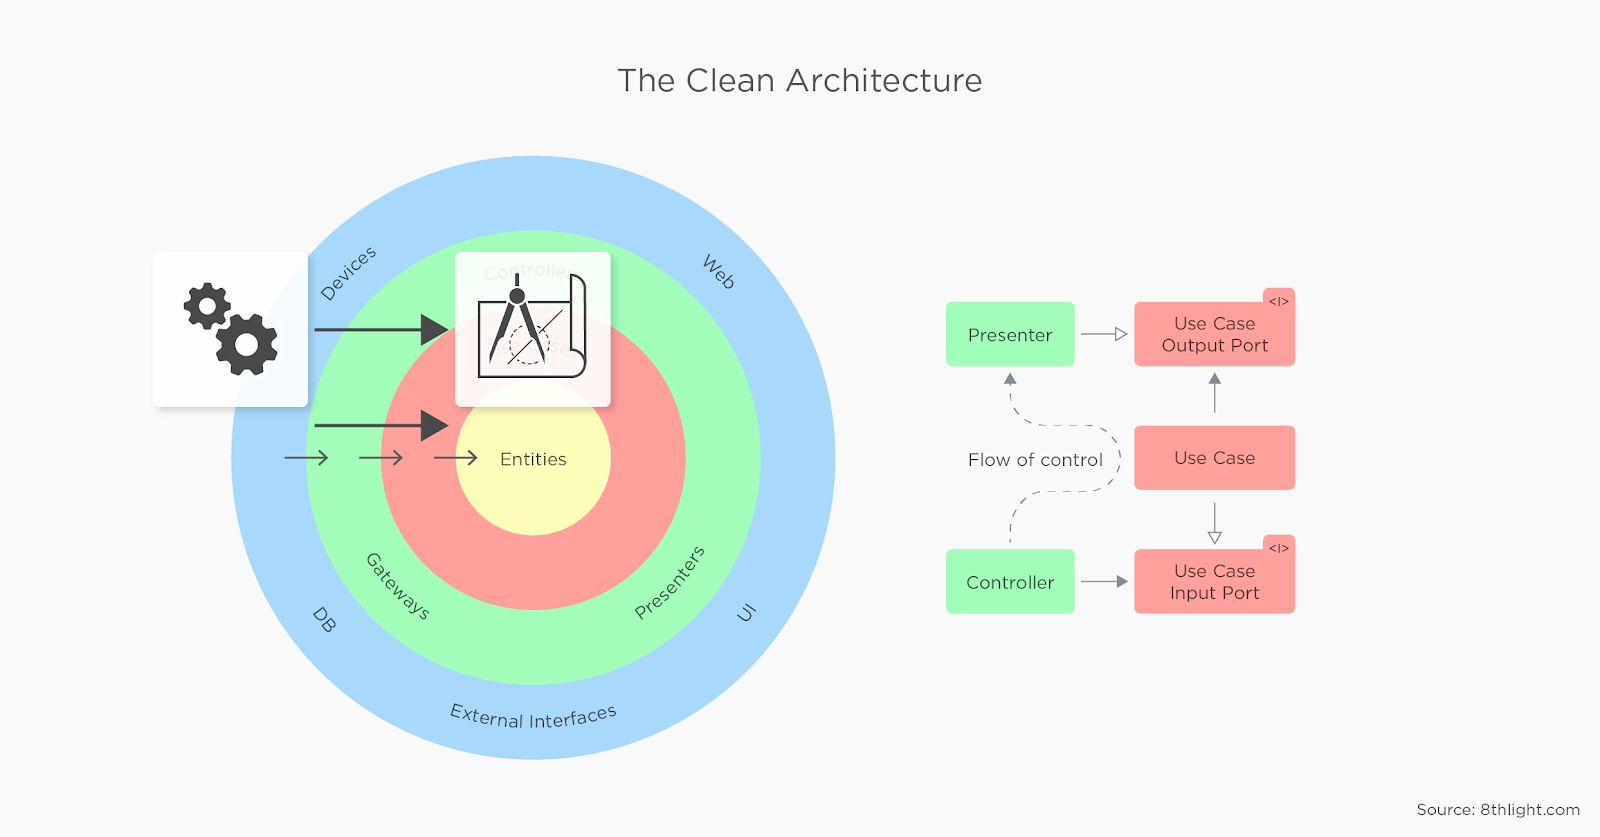
\includegraphics[width=1\textwidth]{Figures/-003.png}
	\rule{35em}{1pt}
	\caption[Abstraction Principle]{Principio de Abstracción en una arquitectura por capas.}
	\label{fig:C2_PA_02}
\end{figure}

\subsection{Comunicación entre Capas}
La lógica del negocio está en el centro del diagrama y debe mediar entre los sistemas externos de salida y los sistemas externos de entrada como la interfaz de usuario, pero ni siquiera sabe que esos dos tipos existen. Esto es un desafío  de comunicación y flujo de datos. Necesitamos que los datos sean capaces de fluir de las capas externas a las internas y viceversa, pero la regla de dependencia no lo permite.

Solo tenemos dos capas, la verde y la roja. La capa verde es exterior y sabe sobre la capa roja, la roja es interior y solo se conoce a sí mismo. Necesitamos que los datos fluyan desde el verde al rojo y viceversa. La solución propuesta se muestra en el diagrama ~\ref{fig:C2_CC_01}:

\begin{figure}[htbp]
	\centering
	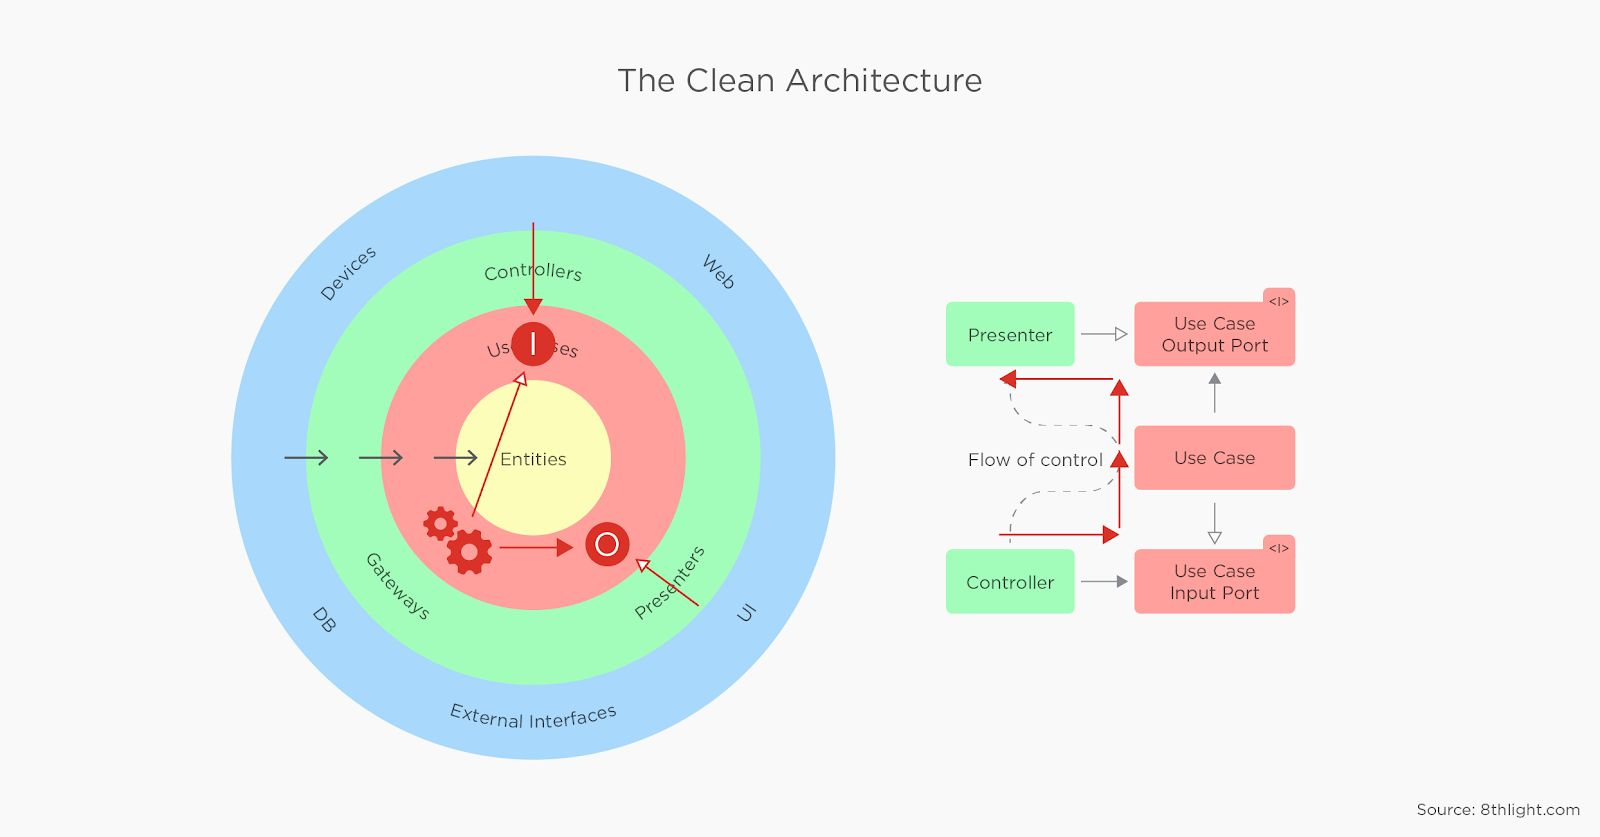
\includegraphics[width=1\textwidth]{Figures/-004.png}
	\rule{35em}{1pt}
	\caption[Layer Communication]{Comunicación entre capas.}
	\label{fig:C2_CC_01}
\end{figure}

En la parte inferior derecha del diagrama ~\ref{fig:C2_CC_01} muestra el flujo de datos. Los datos van desde el controlador, a través del puerto de entrada del caso de uso (o reemplazar el caso de uso con el componente de su elección), luego a través del propio caso de uso y después a través del puerto de salida del caso de uso al presentador.

El controlador tiene un puerto de entrada, literalmente tiene una referencia a él. Llama a un método en él, de modo que los datos van del controlador al puerto de entrada. Pero el puerto de entrada es una interfaz, y la implementación real es el caso de uso: por lo que ha llamado un método en un caso de uso y los flujos de datos al caso de uso. El caso de uso hace algo y quiere enviar los datos de vuelta. Tiene una referencia al puerto de salida, ya que el puerto de salida está definido en la misma capa, por lo que puede llamar al método en él. Por lo tanto, los datos van al puerto de salida. Y finalmente, el presentador es, o implementa, el puerto de salida.
\subsection{Diseño de las Capas}

Los mejores intentos de implementación para proyectos android de esta arquitectura vienen de la mano de un desarrollador argentino Fernando Cejas \cite{clean_cejas} (SoundCloud) y los ejemplos de los Blueprints de arquitectura de  Google\cite{clean_android_blueprints}.\\
Ambas propuestas dividen la implementación en tres capas principales, una capa de presentación, una capa de dominio y la capa de datos.
Cada una de estas capas tiene una responsabilidad bien definida y se comunica con una única capa respetando la regla de dependencia establecida anteriormente cuando se definían los lineamientos generales de la arquitectura.
La cadena de dependencias puede apreciarse en la figura ~\ref{fig:Diagrama_clasico2} la capa de presentación le comunica las demandas del usuario a partir de las interacciones recibidas a la capa de dominio que a su vez realiza las solicitudes de datos a la capa de datos que una vez resueltos le comunica los resultados a la capa de dominio que ejecutará la lógica de negocios pertinente generando una respuesta que producirá los efectos deseados en la capa de presentación.\\
\begin{figure}[htbp]
	\centering
	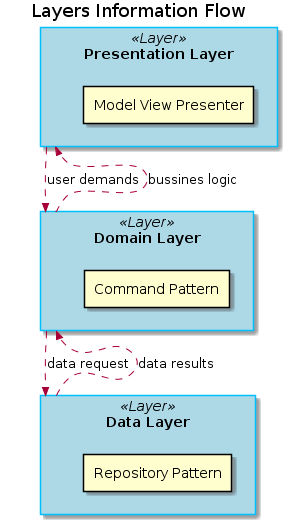
\includegraphics[width=0.3\textwidth]{Figures/-006.png}
	\rule{35em}{1pt}
	\caption[Dependencia de Módulos]{Esquema de dependencias para una arquitectura en capas.}
	\label{fig:Diagrama_clasico2}
\end{figure}
A continuación se describe brevemente las responsabilidades de cada capa.




\begin{itemize}
	\item Presentation Layer: Esta capa se encarga de presentar la interfaz de usuario, esto es, mostrar por pantalla los objetos visuales correspondientes y recibir los eventos de interacción que realiza el usuario. Para la implementación se recomienda el empleo del patrón de diseño conocido como \textbf{MVP (Model View Presenter)}. 
	\item Domain Layer: Esta capa contiene toda la lógica de negocio. La capa de dominio contiene las clases denominadas casos de uso o interactores según la literatura. Estos objetos encapsulan los escenarios contemplados por la lógica de negocio y son ejecutados por la capa de presentación. Estos casos de uso representan todas las acciones posibles admitidas por el sistema y que pueden ser compuestas en la implementación por los desarrolladores siempre desde la capa de presentación. Para la implementación de estos casos de uso se sugiere la utilización del patrón de diseño conocido como \textbf{Command Pattern}.
	\item Data Layer: Esta capa administra la adquisición de datos y es capaz de utilizar diferentes orígenes de datos, así como la lógica de cache o persistencia temporal. Esta capa se suele implementar utilizando el patrón de diseño conocido como \textbf{Repository Pattern}.  
\end{itemize}

\subsection{Presentation Layer: MVP}
El patrón de arquitectura que se utiliza en la capa de presentación de ambas implementaciones se conoce como Modelo-Vista-Presentador.
La idea detrás del patrón es concentrar la lógica de la interacción con el usuario en una entidad conocida como presentador, las operaciones directamente relacionadas con la manipulación de objetos gráficos y la captura de acciones de usuario están delegadas a la entidad Vista, finalmente la adquisición de datos y la ejecución de los algoritmos que encapsulan la lógica de negocio forman parte de las entidades modelo en el patrón \cite{mvp_leiva}.
El diagrama de componentes ~\ref{fig:uml_mvp_component} describe la relación entre los objetos principales propuestos por el patrón.

\begin{figure}[htbp]
	\centering
	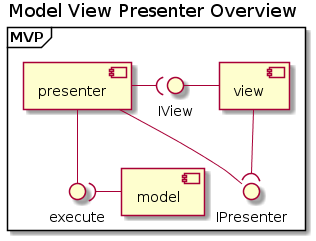
\includegraphics[width=0.5\textwidth]{Figures/uml_mvp_component.png}
	\rule{35em}{1pt}
	\caption[MVP Components]{Diagrama de componentes del patrón.}
	\label{fig:uml_mvp_component}
\end{figure}

Es posible deducir el esquema de comunicación entre los componentes a partir del diagrama. La vista se comunica de manera bidireccional con el presentador y cuando es necesario el presentador se comunica de manera unidireccional con el modelo.


Una convención para la implementación del patrón es tratar de generar vistas completamente ajenas de cualquier lógica operativa y agnósticas del estado de la aplicación. Esto las convierte en un mero instrumento de interfaz entre lo que percibe el usuario y sus reacciones. 

Otra de las convenciones sugiere utilizar objetos modelo-vista en la comunicación entre el presentador y la vista para estandarizar el tipo de mensaje y el proceso de actualización de la vista.

En el caso de las implementaciones antes mencionadas la interfaz con el modelo es satisfecha mediante el uso de objetos casos de uso ó interactores, ambos términos suelen utilizarse de manera intercambiable.

La secuencia de mensajes que son intercambiados entre los objetos del patrón se ilustran en el diagrama de secuencias ~\ref{fig:uml_mvp_sequence}

\begin{figure}[htbp]
	\centering
	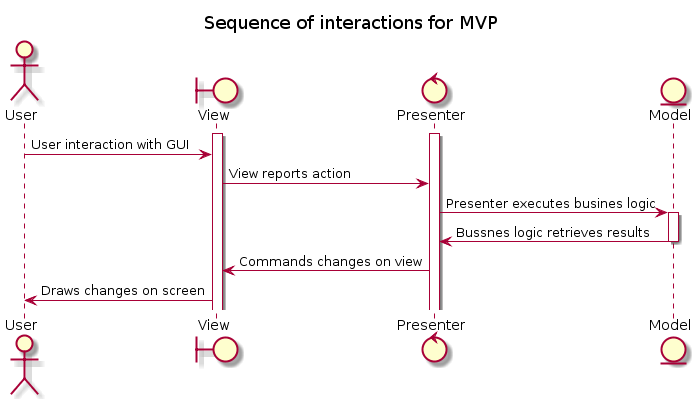
\includegraphics[width=0.7\textwidth]{Figures/uml_mvp_sequence.png}
	\rule{35em}{1pt}
	\caption[MVP Sequence]{Diagrama de secuencia para una interacción con el usuario utilizando MVP.}
	\label{fig:uml_mvp_sequence}
\end{figure}

\subsection{Domain Layer: Commander Pattern}
El patrón de diseño conocido como Commander se utiliza para abstraer la ejecución de procedimientos mediante la implementación de entidades comando \cite{comm_sugrue}. Estos objetos ejecutan un único algoritmo y encapsulan la lógica de negocio de la aplicación o sistema.
Originalmente el diseño contempla 4 entidades principales que se pueden apreciar en el diagrama de clases de la figura ~\ref{fig:uml_clases_commander}:

\begin{figure}[htbp]
	\centering
	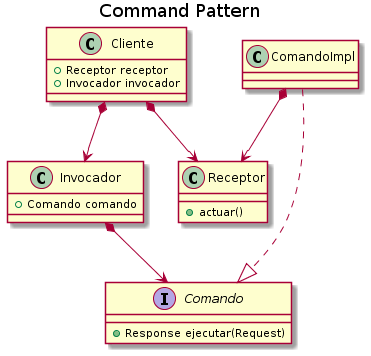
\includegraphics[width=0.6\textwidth]{Figures/uml_clases_commander.png}
	\rule{35em}{1pt}
	\caption[Commander Classes]{Diagrama de clases para el planteo inicial del patrón Commander.}
	\label{fig:uml_clases_commander}
\end{figure}

\begin{enumerate}
	\item Cliente: Este componente se encarga de crear las instancias de cada comando y distribuirlas entre los correspondientes invocadores.
	\item Receptor: Es la entidad que se ve afectada por la ejecución de un comando. Puede ser compartida por varios comandos o bien un único comando puede interactuar con varios receptores en su ejecución.
	\item Comando: Esta entidad contiene la implementación del algoritmo o lógica de ejecución.
	\item Invocador: Se encarga de ejecutar instancias de comandos.
\end{enumerate}

\begin{figure}[htbp]
	\centering
	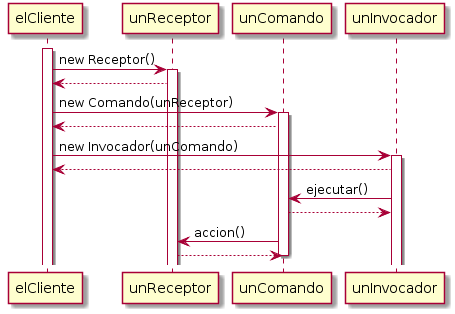
\includegraphics[width=0.7\textwidth]{Figures/uml_sequence_commander.png}
	\rule{35em}{1pt}
	\caption[MVP Components]{Diagrama de secuencia para el patrón Commander.}
	\label{fig:uml_commander_sequence}
\end{figure}

El enfoque inicial sugiere la implementación de un comando
por cada una de las operaciones soportadas por el sistema o aplicación. Sin embargo en sistemas suficientemente grandes la diversidad de funcionalidades soportadas es tan grande que el diseño propuesto se vuelve impráctico.
Para mitigar este problema se suele implementar de manera adicional una modificación que permite la ejecución paramétrica de los comandos para reducir al máximo la cantidad de comandos implementados.
Esta modificación permite diversas alternativas de implementación pero la más utilizada es incorporar conceptos del patrón Request-Response dónde el caso de uso se trata como una entidad de caja negra que admite Solicitudes y emite Respuestas estandarizadas para cada caso.
\begin{itemize}
	\item Solicitud (Request): Un objeto que contiene el conjunto de parámetros de entrada que deben ser satisfechos para poder realizar la ejecución de la rutina del comando.
	\item Respuesta (Response): Un objeto que contiene los valores que se obtuvieron de la ejecución del algoritmo del comando.
\end{itemize}

Por lo tanto puede inferirse el flujo de operación y ejecución de los comandos.

\begin{enumerate}
	\item El cliente crea instancias de comandos y sus correspondientes invocadores. 
	\item El invocador crea e inicializa los objeto solicitud necesarios para ejecutar cada comando.
	\item El invocado ejecuta los comandos llamando al método ''ejecutar'' implementado por cada comando pasando como parámetro la solicitud previamente creada.
	\item El invocador observa los resultados en espera activa implementando el patrón Observer o mediante algún esquema de callback.
\end{enumerate}

\begin{figure}[htbp]
	\centering
	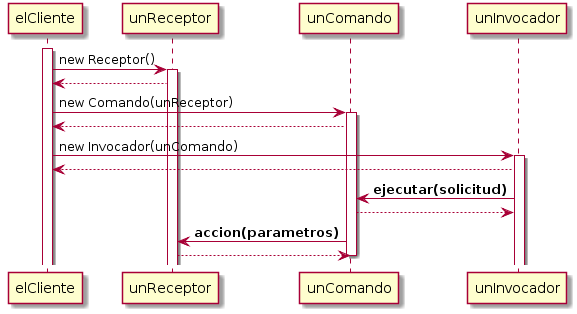
\includegraphics[width=0.8\textwidth]{Figures/uml_sequence_commander_req_resp.png}
	\rule{35em}{1pt}
	\caption[Commander Review]{Diagrama de secuencia para el diseño revisado.}
	\label{fig:uml_commander_sequence_req_resp}
\end{figure}

Siguiendo los lineamientos de la arquitectura propuesta los autores denominan a los comandos: Casos de Uso, ó Interactores.

Como una nota relevante de implementación se recomienda ejecutar las rutinas de los comandos en un hilo/proceso separado para para evitar bloquear el proceso principal de la aplicación.



\subsection{Data Layer: Repository Pattern}
En la capa de datos se propone la implementación de un patrón de diseño conocido como Repository(Repositorio). 
Originalmente se concibe a este diseño como una forma de estandarizar la implementación y el uso de los objetos DAO (Data Access Object) comúnmente utilizados para mapear objetos entidad con las persistencias en la base de datos \cite{repo_wolf}.
Adicionalmente este patrón encapsula en la clase repositorio todos los métodos particulares de filtrado, procesamiento calculado y ordenamiento de entidades.
Sin embargo se define una interfaz genérica que deberá ser respetada por todas las implementaciones de repositorios para todo el sistema independientemente de la entidad que atienda.
En el diagrama de clases de la figura ~\ref{fig:uml_clases_repository} se puede apreciar el diseño original del patrón.

\begin{figure}[htbp]
	\centering
	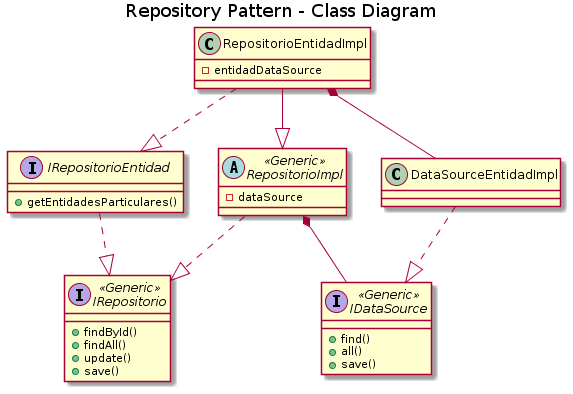
\includegraphics[width=0.8\textwidth]{Figures/uml_clases_repository.png}
	\rule{35em}{1pt}
	\caption[Repository Pattern Class Diagram]{Diagrama de clases del patrón Repository.}
	\label{fig:uml_clases_repository}
\end{figure}

Como puede apreciarse en el diagrama se definen:
\begin{itemize}
	\item IRepositorio: es una interfaz genérica que establece el contrato básico que deben respetar todas las implementaciones de repositorios.
	\item RepositorioImpl: es una clase genérica que establece la interacción con una fuente de datos genérica.
	\item IRepositorioEntidad: es la interfaz que \textit{Especifica} la interfaz genérica de repositorio y establece el contrato o métodos particulares que deberá cumplir la implementación concreta de repositorio para esta Entidad en particular.
	\item RepositorioEntidadImpl: es la clase que \textit{Especifica} la implementación genérica de repositorio e implementa los métodos particulares para esta Entidad en particular.
\end{itemize}

En una repaso más detallado del diagrama puede observarse que existen dos interfaces genéricas para acceso de datos IRepository y IDataSource, esto podría generar confusión y generar duplicación de código. Adicionalmente en cualquier implementación moderna de sistemas con persistencia es prácticamente mandatorio el empleo de frameworks que soportan ORM (Object Relational Mapping) out-of-the-box.
En la figura ~\ref{fig:uml_clases_detalles_repository} se puede observar la modificación sobre la propuesta original del patrón de diseño.

\begin{figure}[htbp]
	\centering
	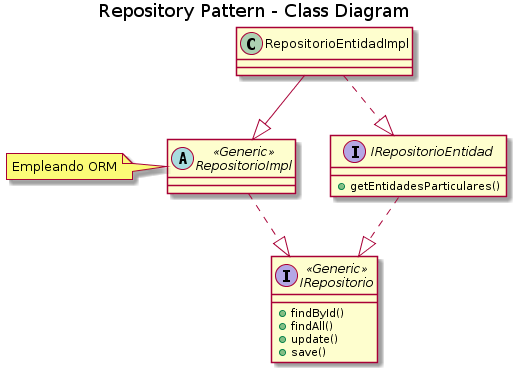
\includegraphics[width=0.8\textwidth]{Figures/uml_clases_nodatasources_repository.png}
	\rule{35em}{1pt}
	\caption[Repository Pattern Detailed Class Diagram]{Diagrama de clases detallado del patrón Repository.}
	\label{fig:uml_clases_detalles_repository}
\end{figure}

Por lo antes expuesto parece razonable plantear una fusión entre el concepto de repositorio y fuente de datos. Coloquialmente es fácil de entender ya que un repositorio definitivamente es una fuente de datos. Si además se quita la estandarización por genéricos se consigue un diseño más sencillo y que genera menos código estructural o scafold manteniendo un único contrato o interfaz de acceso a los datos. En la figura ~\ref{fig:uml_clases_modif_repository} se puede observar la modificación mencionada y el diseño final propuesto para la implementación del patrón.


\begin{figure}[htbp]
	\centering
	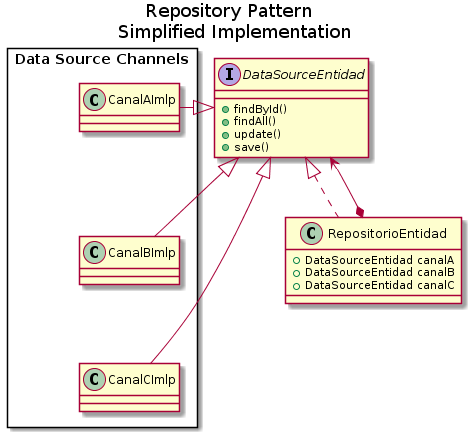
\includegraphics[width=0.5\textwidth]{Figures/uml_clases_modif_repository.png}
	\rule{35em}{1pt}
	\caption[Modified Repository Pattern Class Diagram]{Diagrama de clases del patrón Repository modificado.}
	\label{fig:uml_clases_modif_repository}
\end{figure}

Principalmente orientado a encapsular la manipulación, selección, priorización y mantenimiento de diversas fuentes u orígenes de datos, este esquema de repositorios modificado permite que el peticionario se comunique con una única interfaz para solicitar operaciones sobre datos permaneciendo agnóstico del origen de datos sobre el cual tendrán impacto. 
Implementar una política de caching local se convierte en una tarea sencilla de implementar y mantener.
Esta es la implementación del patrón que se observó en los códigos estudiados.

\section{Programación Reactiva}

La programación reactiva es un paradigma de programación basado en la gestión de flujos de datos asíncronos (streams) y en la propagación del cambio.
Este paradigma está enfocado en el trabajo con flujos de datos finitos o infinitos de manera asíncrona, permitiendo que estos datos se propaguen generando cambios en la aplicación, es decir, ''reaccionan'' a los datos ejecutando una serie de eventos.
Su principal característica es el uso de llamadas asíncronas no bloqueantes siempre que sea posible. Esto incluye no sólo las habituales llamadas a recursos muy lentos a través de la red, sino a todo aquello que sea posible, como las llamadas a base de datos, la gestión de peticiones y en general todo el flujo de llamadas.
La mayoría de los lenguajes de programación más populares soportan este paradigma de programación a través de la inclusión de librerías estándar que implementan internamente el patrón de diseño Observer para la definición de los objetos emisores de eventos (streams) y los consumidores o observadores (subscribers) que son notificados cada vez que se produce un evento.
Adicionalmente suelen implementar el patrón Itarator para convertir colecciones de datos en flujos asíncoronos o streams.
\subsection{Patrón Observer}
Según este patrón, hay un sujeto que es el productor de la información (stream) y por otro lado hay uno o varios consumidores de esta información. En java, por ejemplo, el sujeto sería el objeto Observable y el consumidor el objeto  Suscriber.
Los observables son los encargados de propagar la información y notificar sus cambios, para ello proporciona métodos a partir de los cuales los consumidores pueden suscribirse o cancelar la suscripción de sus flujos de datos.
Los consumidores, por su parte, deciden cuándo quiere suscribirse o cancelar la suscripción a un sujeto, además, ellos mismos son los encargados de actualizar su propio estado cuando el sujeto les notifica de un cambio en el stream de datos. En la figura ~\ref{fig:uml_class_observer} se muestra el diagrama de clases del patrón observer.
\begin{figure}[htbp]
	\centering
	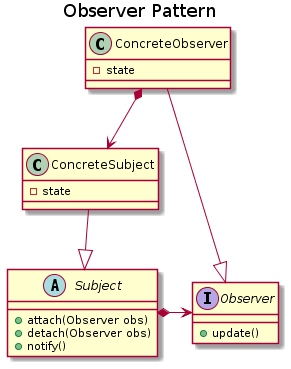
\includegraphics[width=0.3\textwidth]{Figures/uml_class_observer.png}
	\rule{35em}{1pt}
	\caption[Observer Class Diagram]{Diagrama de clases del patrón Observer.}
	\label{fig:uml_class_observer}
\end{figure}
\subsection{Patrón Iterator}
El patrón iterador nos permite recorrer contenedores de información, por ejemplo un arreglo o una lista de objetos sin necesidad de conocer el tipo de contenido o el tamaño de la colección de objetos. En la figura ~\ref{fig:uml_class_iterator} se muestra el diagrama de clases tradicional de su implementación.
\begin{figure}[htbp]
	\centering
	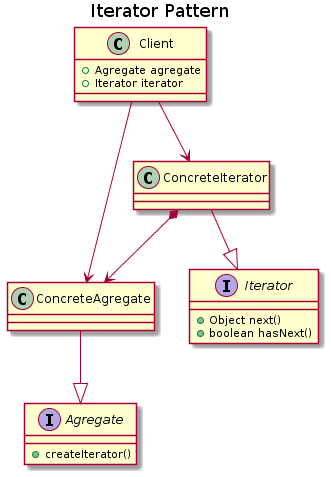
\includegraphics[width=0.4\textwidth]{Figures/uml_class_iterator.png}
	\rule{35em}{1pt}
	\caption[Iterator Class Diagram]{Diagrama de clases del patrón Iterador.}
	\label{fig:uml_class_iterator}
\end{figure}

\subsection{Programación Reactiva y Clean Architecture}
Aplicando programación reactiva es posible observar un sentido deliberado del flujos de datos al considerar la dependencia entre las capas definidas por la arquitectura y sus respectivos componentes.
En la figura ~\ref{fig:uml_infflow_modif_repository} se puede apreciar este flujo de dato en las flehas azules que indican el intercambio de datos. Las flechas rojas indican las invocaciones.
\begin{figure}[htbp]
	\centering
	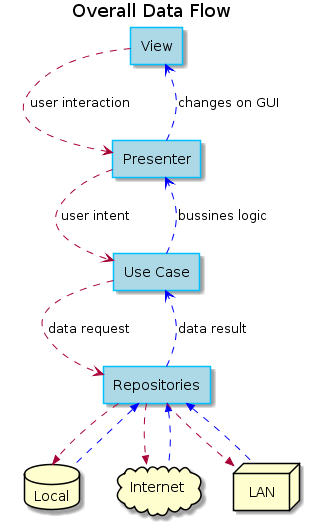
\includegraphics[width=0.4\textwidth]{Figures/uml_inf-flow_clean_reactive.png}
	\rule{35em}{1pt}
	\caption[Modified Repository Pattern Class Diagram]{Diagrama de clases del patrón Repository modificado.}
	\label{fig:uml_infflow_modif_repository}
\end{figure}